\documentclass[a4paper,12pt]{article}

% ─── Кодировка и язык ───
\usepackage[utf8]{inputenc}
\usepackage[T2A]{fontenc}
\usepackage[russian]{babel}

% ─── Поля ───
\usepackage[left=2.5cm, right=1.5cm, top=2cm, bottom=2cm]{geometry}

% ─── Пакеты ───
\usepackage{graphicx}
\usepackage{booktabs}
\usepackage{longtable}
\usepackage{hyperref}
\usepackage{listings}
\usepackage{xcolor}
\usepackage{caption}
\usepackage{enumitem}
\usepackage{float}
\usepackage{tabularx}
\usepackage{verbatim}

% ─── Настройка листингов ───
\lstset{
  basicstyle=\ttfamily\footnotesize,
  backgroundcolor=\color{gray!10},
  frame=single,
  breaklines=true,
  breakatwhitespace=true,
  showstringspaces=false,
  numbers=left,
  numberstyle=\tiny\color{gray},
  keywordstyle=\color{blue!70},
  commentstyle=\color{green!50!black},
  stringstyle=\color{red!60},
}

\hypersetup{
  colorlinks=true,
  linkcolor=blue!60!black,
  urlcolor=blue!70!black,
  citecolor=green!50!black
}

\usepackage{setspace}
\onehalfspacing

\begin{document}

% ═══════════════════════════════════════════
% ТИТУЛЬНЫЙ ЛИСТ
% ═══════════════════════════════════════════

\begin{titlepage}
\begin{center}

\textbf{РОССИЙСКИЙ УНИВЕРСИТЕТ ДРУЖБЫ НАРОДОВ\\ИМЕНИ ПАТРИСА ЛУМУМБЫ}\\[0.3cm]
\textbf{Факультет физико-математических и естественных наук}\\[0.3cm]
Направление подготовки: 09.03.03 <<Прикладная информатика>>\\[2cm]

{\Large \textbf{ЗАДАНИЕ 6П}}\\[0.5cm]
{\large \textbf{Программный комплекс на GitHub}}\\[1cm]

{\large Тема НИР:}\\[0.3cm]
{\large <<Анализ тональности сообщений пользователей социальных сетей\\
и оценка их влияния на динамику цен криптовалют>>}\\[2cm]

\begin{tabular}{ll}
\textbf{Студент:} & Мугари Абдеррахим \\
\textbf{Группа:} & НФИбд-01-22 \\
\textbf{Науч. рук.:} & доц., к.т.н. Молодченков А.И. \\
\textbf{Трек:} & П (прикладной) \\
\end{tabular}

\vfill
Москва, 2026

\end{center}
\end{titlepage}

\tableofcontents
\newpage

% ═══════════════════════════════════════════
% 1. РЕПОЗИТОРИЙ
% ═══════════════════════════════════════════

\section{Репозиторий проекта}

Код проекта размещён в открытом репозитории на GitHub:

\begin{center}
\url{https://github.com/iragoum/nlp-crypto-sentiment-pipeline}
\end{center}

\subsection{Структура репозитория}

\begin{lstlisting}[language={}, caption={Структура каталогов проекта}]
nlp-crypto-sentiment-pipeline/
|-- .github/workflows/ci.yml    # CI/CD pipeline
|-- data/
|   |-- raw/                    # Исходные данные (tweets.csv)
|   |-- processed/              # Обработанные данные
|-- src/
|   |-- __init__.py
|   |-- data_loader.py          # Загрузка и валидация данных
|   |-- preprocessor.py         # Предобработка текста
|   |-- sentiment_analyzer.py   # VADER + FinBERT
|   |-- price_fetcher.py        # Получение цен CoinGecko
|   |-- correlation_analyzer.py # Корреляции и каузальность
|-- tests/
|   |-- __init__.py
|   |-- test_preprocessor.py
|   |-- test_sentiment_analyzer.py
|   |-- test_correlation_analyzer.py
|-- results/
|   |-- figures/                # Графики (PNG)
|   |-- tables/                 # Таблицы (CSV)
|   |-- finbert_torchinfo.txt   # Архитектура модели
|   |-- finbert_architecture.onnx  # ONNX-экспорт
|-- main.py                     # Точка входа pipeline
|-- requirements.txt            # Зависимости (полные)
|-- requirements-test.txt       # Зависимости для тестов
|-- README.md                   # Документация
\end{lstlisting}

% ═══════════════════════════════════════════
% 2. ОПИСАНИЕ МОДУЛЕЙ
% ═══════════════════════════════════════════

\section{Описание программных модулей}

\subsection{\texttt{src/data\_loader.py}}

Модуль отвечает за загрузку и валидацию датасета Twitter-сообщений.

\begin{itemize}
  \item \texttt{load\_tweets(path, lang\_filter)} --- загрузка CSV, фильтрация по языку,
        проверка наличия обязательных колонок (\texttt{full\_text}, \texttt{date}).
\end{itemize}

\subsection{\texttt{src/preprocessor.py}}

Модуль предобработки текста.

\begin{itemize}
  \item \texttt{clean\_text(text)} --- удаление URL, упоминаний, RT-префикса,
        не-ASCII символов, приведение к нижнему регистру.
  \item \texttt{tokenize(text, remove\_stopwords)} --- NLTK-токенизация,
        фильтрация стоп-слов.
  \item \texttt{preprocess\_dataframe(df)} --- применение предобработки
        ко всему DataFrame, добавление колонок \texttt{cleaned\_text} и \texttt{tokens}.
\end{itemize}

\subsection{\texttt{src/sentiment\_analyzer.py}}

Модуль анализа тональности.

\begin{itemize}
  \item \texttt{score\_vader(texts)} --- VADER-анализ оригинального текста.
        Возвращает: compound, pos, neg, neu.
  \item \texttt{score\_finbert(texts, batch\_size)} --- FinBERT-классификация
        очищенного текста. Возвращает: label (positive/neutral/negative), score.
  \item \texttt{get\_torchinfo\_summary()} --- вывод архитектуры модели через torchinfo.
  \item \texttt{export\_onnx(output\_path)} --- экспорт модели в формат ONNX.
\end{itemize}

\subsection{\texttt{src/price\_fetcher.py}}

Модуль получения ценовых данных.

\begin{itemize}
  \item \texttt{fetch\_prices(coin\_id, start, end)} --- запрос к CoinGecko API
        с 3 повторными попытками.
  \item \texttt{get\_fallback\_prices()} --- встроенные исторические данные BTC
        (июль--август 2022) для offline-режима.
  \item \texttt{load\_or\_fetch\_prices()} --- кэширование с автоматическим fallback.
\end{itemize}

\subsection{\texttt{src/correlation\_analyzer.py}}

Модуль статистического анализа.

\begin{itemize}
  \item \texttt{aggregate\_daily\_sentiment(df)} --- агрегация tweet-level $\rightarrow$
        daily-level метрик тональности.
  \item \texttt{compute\_lagged\_correlations(merged, sent, price, max\_lag)} ---
        расчёт корреляций Пирсона и Спирмена при лагах 0--7 дней.
  \item \texttt{run\_granger\_test(merged, sent, price, max\_lag)} ---
        тест Грейнджер-каузальности (F-статистика, p-value).
  \item \texttt{adf\_test(series, name)} --- расширенный тест Дики--Фуллера.
  \item \texttt{correlation\_matrix(merged, cols, method)} --- матрица корреляций.
\end{itemize}

\subsection{\texttt{main.py}}

Точка входа pipeline. Последовательно выполняет все этапы анализа,
генерирует таблицы и графики, поддерживает CLI-аргументы:

\begin{itemize}
  \item \texttt{-{}-skip-finbert} --- пропуск FinBERT (только VADER);
  \item \texttt{-{}-skip-torchinfo} --- пропуск вывода архитектуры;
  \item \texttt{-{}-sample N} --- подвыборка N твитов;
  \item \texttt{-{}-coin} --- идентификатор криптовалюты (по умолчанию: bitcoin).
\end{itemize}

% ═══════════════════════════════════════════
% 3. ДОКУМЕНТАЦИЯ КОДА
% ═══════════════════════════════════════════

\section{Документация кода}

Все модули и функции документированы с помощью docstrings в формате Google-style.
Каждая функция содержит:

\begin{enumerate}
  \item Описание назначения функции.
  \item Раздел \texttt{Args} с типами и описанием каждого параметра.
  \item Раздел \texttt{Returns} с описанием возвращаемого значения.
\end{enumerate}

Типы аргументов указаны с использованием type hints (PEP 484):

\begin{lstlisting}[language=Python, caption={Пример документированной функции}]
def load_tweets(path: str | Path,
                lang_filter: str = "en") -> pd.DataFrame:
    """Load and validate the tweet dataset.

    Args:
        path: Path to the CSV file.
        lang_filter: ISO language code to keep.

    Returns:
        DataFrame with columns: id, created_at,
        date, full_text, retweet_count, favorite_count.
    """
\end{lstlisting}

% ═══════════════════════════════════════════
% 4. CI/CD
% ═══════════════════════════════════════════

\section{Непрерывная интеграция (CI/CD)}

Настроен workflow GitHub Actions (\texttt{.github/workflows/ci.yml}),
который автоматически запускается при каждом push или pull request в ветку \texttt{main}.

\subsection{Конфигурация}

\begin{itemize}
  \item \textbf{Матрица версий:} Python 3.10, 3.11, 3.12.
  \item \textbf{Зависимости:} \texttt{requirements-test.txt} (облегчённый набор без torch/transformers).
  \item \textbf{Шаги:}
    \begin{enumerate}
      \item Установка Python и кэширование pip-пакетов.
      \item Установка зависимостей.
      \item Загрузка данных NLTK (stopwords, punkt, punkt\_tab).
      \item Запуск тестов (\texttt{pytest tests/ -v}).
      \item Линтинг (\texttt{flake8}).
    \end{enumerate}
\end{itemize}

\subsection{Статус}

Все проверки проходят успешно на всех трёх версиях Python.

% ═══════════════════════════════════════════
% 5. АРХИТЕКТУРА НЕЙРОННОЙ СЕТИ
% ═══════════════════════════════════════════

\section{Архитектура нейронной сети (FinBERT)}

\subsection{Описание модели}

FinBERT (ProsusAI/finbert) --- модель на основе архитектуры BERT
(Bidirectional Encoder Representations from Transformers),
дообученная на корпусе финансовых текстов для задачи классификации тональности
на 3 класса: positive, neutral, negative.

\subsection{Вывод torchinfo}

Вывод архитектуры модели с помощью библиотеки torchinfo сохранён
в файле \texttt{results/finbert\_torchinfo.txt}:

\begin{lstlisting}[language={}, caption={Архитектура FinBERT (torchinfo)}, basicstyle=\ttfamily\scriptsize]
==========================================================================
Layer (type:depth-idx)          Input Shape       Output Shape   Param #
==========================================================================
BertForSequenceClassification   --                [1, 3]         --
|--BertModel: 1-1               [1, 128]          [1, 768]       --
|  |--BertEmbeddings: 2-1       --                [1,128,768]    --
|  |  |--Embedding: 3-1         [1, 128]          [1,128,768]    23,440,896
|  |  |--Embedding: 3-2         [1, 128]          [1,128,768]    1,536
|  |  |--Embedding: 3-3         [1, 128]          [1,128,768]    393,216
|  |  |--LayerNorm: 3-4         [1,128,768]       [1,128,768]    1,536
|  |  |--Dropout: 3-5           [1,128,768]       [1,128,768]    --
|  |--BertEncoder: 2-2          [1,128,768]       [1,128,768]    --
|  |  |--ModuleList: 3-6 (x12)  --               --             85,054,464
|  |--BertPooler: 2-3           [1,128,768]       [1, 768]       --
|  |  |--Linear: 3-7            [1, 768]          [1, 768]       590,592
|  |  |--Tanh: 3-8              [1, 768]          [1, 768]       --
|--Dropout: 1-2                 [1, 768]          [1, 768]       --
|--Linear: 1-3 (classifier)     [1, 768]          [1, 3]         2,307
==========================================================================
Total params:            109,484,547
Trainable params:        109,484,547
Non-trainable params:    0
Params size (MB):        437.94
Estimated Total Size:    544.90 MB
==========================================================================
\end{lstlisting}

\subsection{Ключевые характеристики}

\begin{table}[H]
\centering
\caption{Параметры архитектуры FinBERT}
\label{tab:finbert_arch}
\begin{tabular}{|l|c|}
\hline
\textbf{Характеристика} & \textbf{Значение} \\
\hline
Базовая архитектура & BERT-base \\
\hline
Число слоёв энкодера & 12 \\
\hline
Размерность скрытого состояния & 768 \\
\hline
Число голов внимания & 12 \\
\hline
Общее число параметров & 109\,484\,547 \\
\hline
Размер модели & 437.94 MB \\
\hline
Число выходных классов & 3 (positive, neutral, negative) \\
\hline
Максимальная длина входа & 512 токенов \\
\hline
\end{tabular}
\end{table}

\subsection{Визуализация архитектуры (Netron)}

Модель экспортирована в формат ONNX (\texttt{results/finbert\_architecture.onnx})
и визуализирована с помощью инструмента Netron (\url{https://netron.app}).

\begin{figure}[H]
\centering
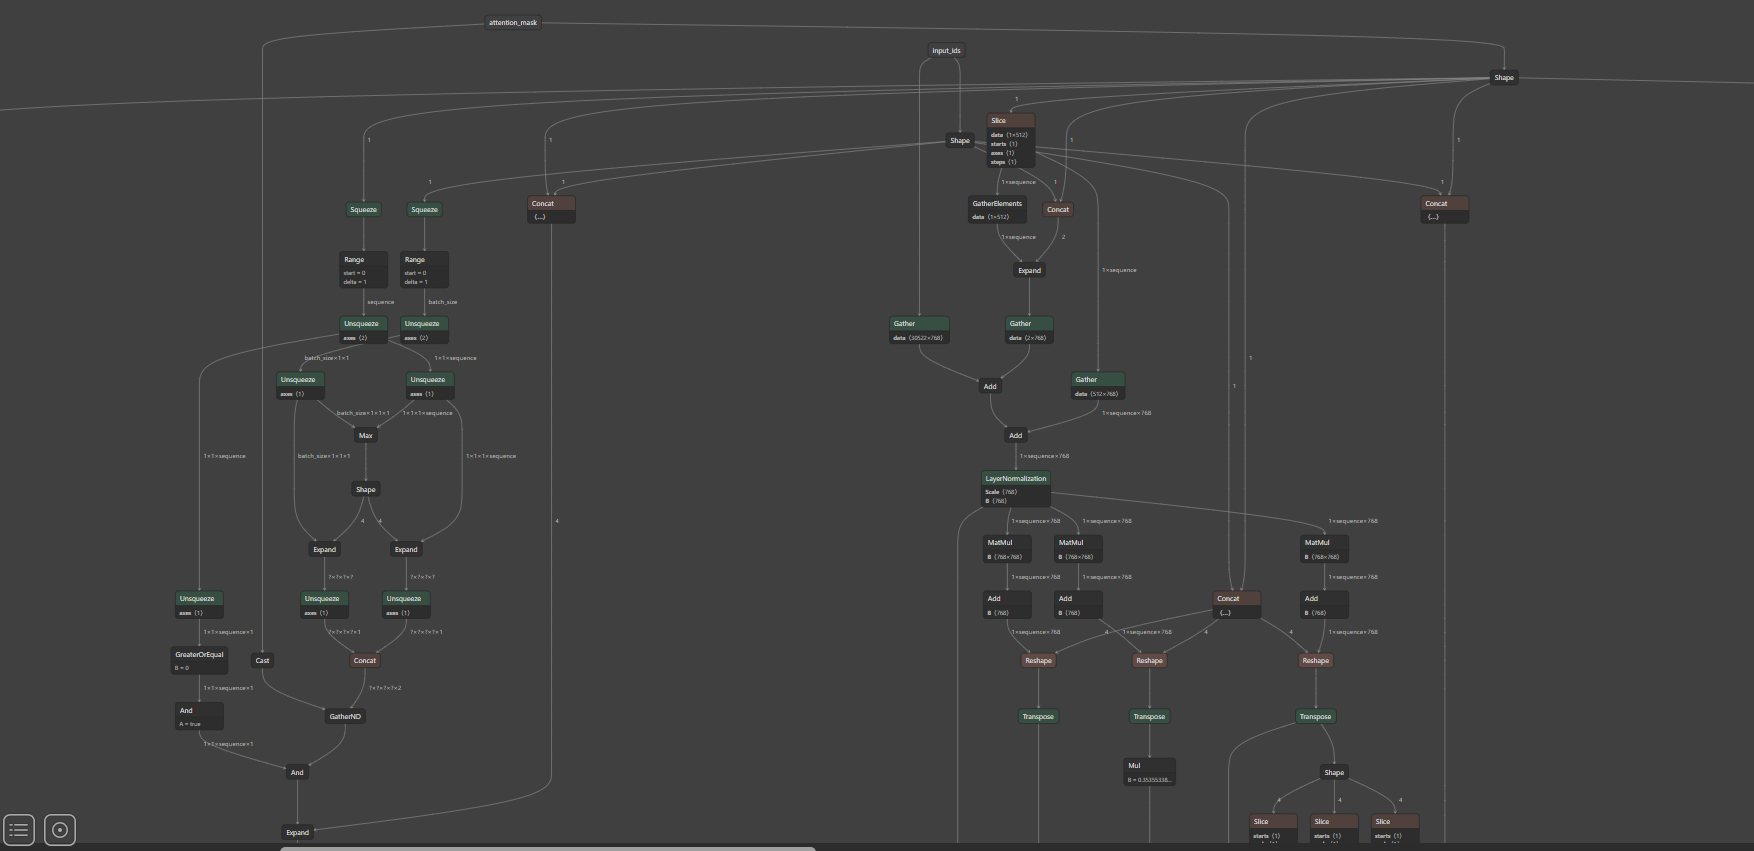
\includegraphics[width=0.9\textwidth]{../results/figures/netron_finbert_small.png}
\caption{Граф архитектуры FinBERT --- верхняя часть (визуализация Netron).
Полный граф доступен в файле \texttt{results/finbert\_architecture.onnx},
который можно открыть на \url{https://netron.app}.}
\label{fig:netron}
\end{figure}

% ═══════════════════════════════════════════
% 6. ВОСПРОИЗВОДИМОСТЬ
% ═══════════════════════════════════════════

\section{Воспроизводимость результатов}

Для обеспечения воспроизводимости результатов:

\begin{enumerate}
  \item Все зависимости зафиксированы в \texttt{requirements.txt}
        с указанием минимальных версий.
  \item Fallback-механизм для ценовых данных обеспечивает работу
        без доступа к CoinGecko API.
  \item Seed (\texttt{random\_state=42}) используется при подвыборке данных.
  \item CI/CD автоматически проверяет работоспособность на трёх версиях Python.
  \item README содержит пошаговую инструкцию по установке и запуску.
\end{enumerate}

\end{document}
